\documentclass[aspectratio=169]{beamer}
\usetheme{metropolis}
\metroset{subsectionpage=progressbar}

\usefonttheme{professionalfonts} % 使用系统/自定字体


% === 字体设置 ===
\usepackage[UTF8,scheme=plain,fontset=none]{ctex}
\setCJKmainfont{Source Han Serif CN}[BoldFont={Source Han Serif CN Bold}]
\setCJKsansfont{Source Han Sans CN}[BoldFont={Source Han Sans CN Bold}]
% \setCJKmonofont{Sarasa Mono CN}

\newcommand{\model}{\epsilon_\theta}
\newcommand{\conditioner}{\tau_\theta}
\newcommand{\zt}[1]{z_{#1}}
\newcommand{\varphii}[1]{\varphi_{#1}}


% beamer 已加载 hyperref;加 unicode 以支持中文书签
\hypersetup{unicode}

% define paragraph
\providecommand{\paragraph}[1]{\smallskip\textbf{#1}\par}

% 常用包
\usepackage{longtable,booktabs}
\usepackage{amsmath,amssymb}
\usepackage{graphicx}
\usepackage{tikz}
\usetikzlibrary{positioning,arrows.meta}
% \graphicspath{{.}{./figs/}{./images/}{./images_in_paper/}}
\usepackage{caption}
\usepackage{subcaption}
\usepackage{float}
\usepackage{svg}
\usepackage{booktabs}
\usepackage{array}
\usepackage{threeparttable}

% 算法环境(与 beamer 兼容)
\usepackage{algorithm}
\usepackage[noend]{algpseudocode}  % 提供 algorithmic 环境、\State 等
% 可选:微调 algorithmic 缩进
\algrenewcommand\algorithmicindent{0.8em}

% 数学粗体与梯度符号
\usepackage{bm} % \boldsymbol
\newcommand{\bx}{\mathbf{x}}
\newcommand{\bz}{\mathbf{z}}
\newcommand{\bI}{\mathbf{I}}
\newcommand{\bzero}{\mathbf{0}}
\newcommand{\bepsilon}{\boldsymbol{\epsilon}}
\newcommand{\grad}{\nabla}
% 超链接(beamer 已加载 hyperref,这里只补选项)
% \hypersetup{unicode=true}

% 编号风格
\setbeamertemplate{caption}[numbered]
\setbeamertemplate{caption label separator}{.}

\title{扩散模型在图像重建与生成任务中的应用}
\author{李孟霖 2311067}
\date{\today}
%---Document Begins---
\begin{document}
\begin{frame}[plain]
  \titlepage
\end{frame}
\section{DDPM}
\begin{frame}
\textbf{Denoising Diffusion Probabilistic Models}

NeruIPS 2020
\end{frame}
\begin{frame}{基本思路}
Denoising Diffusion Probabilistic Models(DDPM)通过逐步添加噪声破坏图像,
再用反向过程逐步去噪重建图像。

模型学习从纯噪声去噪得到图片的过程,从而实现由任意纯高斯噪声生成图片的功能。

该模型结合了变分下界优化和Langevin动力学的去噪得分匹配,实现高质量图像生成。
\end{frame}
\subsection{数学原理}

\begin{frame}{Diffusion Model}
  \textbf{前向过程 (Forward Process)}: \\
  给定原始图像 $x_0 \sim q(x_0)$,前向过程逐步添加高斯噪声,构成一个固定的马尔可夫链:
  \[
    q(x_{1:T} | x_0) = \prod_{t=1}^T q(x_t | x_{t-1}), \quad q(x_t | x_{t-1}) = \mathcal{N}(\sqrt{1 - \beta_t} x_{t-1}, \beta_t I)
  \]
  可直接从 $x_0$ 采样出任意时刻 $x_t$:
  \[
    q(x_t | x_0) = \mathcal{N}(\sqrt{\bar{\alpha}_t} x_0, (1 - \bar{\alpha}_t) I)
  \]
  其中 $\alpha_t = 1 - \beta_t$, $\bar{\alpha}_t = \prod_{s=1}^t \alpha_s$

  \vspace{0.5em}
  \textbf{反向过程 (Reverse Process)}: \\
  从纯噪声 $x_T \sim \mathcal{N}(0, I)$ 开始,反向过程学习一个去噪马尔可夫链:
  \[
    p_\theta(x_{0:T}) = p(x_T) \prod_{t=1}^T p_\theta(x_{t-1} | x_t), \quad p_\theta(x_{t-1} | x_t) = \mathcal{N}(\mu_\theta(x_t, t), \Sigma_\theta(x_t, t))
  \]
  通过神经网络学习均值和方差,实现高质量图像的逐步重建。
\end{frame}

\begin{frame}{DDPM 损失函数构造与简化}

\textbf{目标:} 利用变分下界(ELBO),设计可优化的训练损失函数,以学习从噪声 $x_T$ 逐步生成图像 $x_0$ 的反向过程。

\textbf{1. 变分下界(ELBO)分解:}
\[
  \log p_\theta(x_0) \geq \text{ELBO} = -[L_T + \sum_{t=2}^T L_{t-1} + L_0]
\]
\begin{itemize}
  \item $-L_T$ 是固定常数,可忽略
  \item $-L_{t-1}$ 是主要的训练目标项(KL 散度)
  \item $-L_0$ 是重建项(有时也忽略)
\end{itemize}
\end{frame}

\begin{frame}{DDPM 损失函数构造与简化}
\textbf{2. 反向过程建模为高斯分布:}
\[
p_\theta(x_{t-1}|x_t) = \mathcal{N}(\mu_\theta(x_t, t), \sigma_t^2 I)
\]
\begin{itemize}
  \item 其中 $\sigma_t^2$ 为固定超参数,不学习
  \item $\mu_\theta$ 为模型(如 U-Net)输出
\end{itemize}
\end{frame}
\begin{frame}{DDPM 损失函数构造与简化}
\textbf{3. 损失函数重写为预测后验均值:}
\[
L_{t-1} = \mathbb{E} \left[ \frac{1}{2\sigma_t^2} \| \mu_\theta(x_t, t) - \tilde{\mu}_t(x_t, x_0) \|^2 \right] + C
\]

\textbf{4. 使用重参数化将问题转化为噪声预测:}
\[
x_t = \sqrt{\bar{\alpha}_t} x_0 + \sqrt{1 - \bar{\alpha}_t} \epsilon, \quad \epsilon \sim \mathcal{N}(0, I)
\]

\textbf{最终损失函数简化为:}
\[
\mathcal{L}_{\text{simple}} = \mathbb{E}_{x_0, \epsilon, t} \left[ \left\| \epsilon - \epsilon_\theta(x_t, t) \right\|^2 \right]
\]

\textbf{结论:} 模型训练目标是拟合噪声 $\epsilon$,本质上是一个时间条件的\textbf{去噪任务}。

\end{frame}

\begin{frame}{algorithm}

\algrenewcommand\algorithmicindent{0.5em}%
\begin{figure}[t]
\begin{minipage}[t]{0.495\textwidth}
\begin{algorithm}[H]
  \caption{Training} \label{alg:training}
  \small
  \begin{algorithmic}[1]
    \Repeat
      \State $\bx_0 \sim q(\bx_0)$
      \State $t \sim \mathrm{Uniform}(\{1, \dotsc, T\})$
      \State $\bepsilon\sim\mathcal{N}(\bzero,\bI)$
      \State Take gradient descent step on
      \Statex $\qquad \grad_\theta \left\| \bepsilon - \bepsilon_\theta(\sqrt{\bar\alpha_t} \bx_0 + \sqrt{1-\bar\alpha_t}\bepsilon, t) \right\|^2$
    \Until{converged}
  \end{algorithmic}
\end{algorithm}
\end{minipage}
\hfill
\begin{minipage}[t]{0.495\textwidth}
\begin{algorithm}[H]
  \caption{Sampling} \label{alg:sampling}
  \small
  \begin{algorithmic}[1]
    \vspace{.04in}
    \State $\bx_T \sim \mathcal{N}(\bzero, \bI)$
    \For{$t=T, \dotsc, 1$}
      \State $\bz \sim \mathcal{N}(\bzero, \bI)$ if $t > 1$, else $\bz = \bzero$
      \State $\bx_{t-1} = \frac{1}{\sqrt{\alpha_t}}\left( \bx_t - \frac{1-\alpha_t}{\sqrt{1-\bar\alpha_t}} \bepsilon_\theta(\bx_t, t) \right) + \sigma_t \bz$
    \EndFor
    \State \textbf{return} $\bx_0$
    \vspace{.04in}
  \end{algorithmic}
\end{algorithm}
\end{minipage}
\vspace{-1em}
\end{figure}
\end{frame}

\subsection{模型结构}
\begin{frame}{DDPM 模型结构(U-Net)}
  \begin{figure}[H]
    \centering
    \includegraphics[width=0.9\linewidth]{images/DDPM_UNet.png}
    \caption{DDPM 中用于噪声预测的 U-Net 架构示意图}
  \end{figure}
\end{frame}

\begin{frame}{时间步条件的注入方式}
  \begin{figure}[H]
    \centering
    \includegraphics[width=0.8\linewidth]{images/DDPM_down-up-block.png}
    \caption{U-Net 层内部通过 Add 操作将时间步嵌入融合到特征图中}
  \end{figure}
\end{frame}

\begin{frame}{DDPM 示例}
  \begin{figure}[H]
    \centering
    \includegraphics[width=0.9\linewidth]{./images/stochastic_decoding_single.jpg}
    \caption{DDPM 推理示例}
  \end{figure}
\end{frame}
\section{VAE 压缩模块}

\begin{frame}{VAE 在图像压缩中的核心机制}

\begin{itemize}
  \item \textbf{结构概览}:
  \begin{itemize}
    \item 使用编码器 $E_\phi(x)$ 将高维图像 $x \in \mathbb{R}^{H \times W \times 3}$ 映射为低维潜向量 $z$
    \item 潜空间分布为 $q_\phi(z|x) = \mathcal{N}(\mu(x), \sigma^2(x))$
    \item 解码器 $D_\theta(z)$ 将 $z$ 重建为图像 $\hat{x} = D(z)$
  \end{itemize}

  \item \textbf{压缩意义}:
  \begin{itemize}
    \item $z$ 是图像的紧凑编码,维度远小于原始图像
    \item 潜空间引入正则化(如 KL 散度),避免过度拟合,提升压缩泛化能力
    \item 使用连续高斯向量(而非固定码本),更适合感知一致性场景
  \end{itemize}

  \item \textbf{与传统 Autoencoder 的区别}:
  \begin{itemize}
    \item VAE 学习的是 \textbf{分布} 而非固定编码,压缩后可进行随机采样
    \item 提供更好的鲁棒性与潜变量结构控制
  \end{itemize}

  \item \textbf{压缩 vs 生成}:
  \begin{itemize}
    \item 虽然 VAE 为生成设计,但编码器结构天然适合压缩任务
    \item 实际应用中,如图像重建、感知压缩、表示学习常借助其潜空间能力
  \end{itemize}
\end{itemize}
\end{frame}

\section{Latent Diffusion Model}

\begin{frame}{Latent Diffusion Model (LDM): 功能概览}

\begin{itemize}
  \item \textbf{计算高效}:
  \begin{itemize}
    \item 在\textbf{潜空间(latent space)}中进行扩散建模,避免在高维像素空间中处理。
    \item 显著\textbf{降低训练与推理成本},支持低资源环境运行。
  \end{itemize}

  \item \textbf{灵活的条件生成(Conditional Generation)}:
  \begin{itemize}
    \item 引入 \textbf{Cross-Attention 模块},实现多种输入条件的控制:
    \begin{itemize}
      \item 文本(Text-to-Image)
      \item 边界框(Layout-guided generation)
      \item 掩膜图像(Inpainting)
      \item 类别标签(Class-conditional generation)
    \end{itemize}
  \end{itemize}
  
  \item \textbf{多任务适应性强}:
  \begin{itemize}
    \item 同一模型适用于:
    \begin{itemize}
      \item 无条件图像生成(Unconditional Generation)
      \item 图像修复(Image Inpainting)
      \item 图像增强与重建(e.g., Super-resolution)
    \end{itemize}
  \end{itemize}
\end{itemize}

\end{frame}

\subsection{LDM Autoencoder}
\begin{frame}{LDM 中的 Autoencoder:压缩图像感知结构}

\textbf{目的:} 将图像 $x \in \mathbb{R}^{H \times W \times 3}$ 压缩为结构化潜空间 $z \in \mathbb{R}^{h \times w \times c}$,便于高效训练扩散模型。

\vspace{0.8em}

\textbf{结构组成:}
\begin{itemize}
  \item \textbf{Encoder} $E(x) \rightarrow z$:多层卷积和残差模块(细节参见补充材料或代码)
  \item \textbf{Decoder} $D(z) \rightarrow \tilde{x}$:恢复图像
  \item 下采样比例 $f = H/h = W/w$, 例如 $f = 4, 8, 16$
\end{itemize}

\vspace{0.8em}

\textbf{训练目标:}
\begin{itemize}
  \item 使用 \textbf{感知损失(perceptual loss)}:保持图像语义细节
  \item 使用 \textbf{PatchGAN 对抗损失}:增强局部真实性,避免模糊
  \item 最小化重建误差 $\mathcal{L}_{\text{rec}}(x, \tilde{x})$
\end{itemize}

\end{frame}

\begin{frame}{Autoencoder 的正则化与训练策略}

\textbf{潜空间正则化目的:} 避免高方差、非结构化的 latent 表示,增强生成稳定性。

\vspace{0.6em}

\textbf{两种正则化方式:}
\begin{itemize}
  \item \textbf{KL 正则(KL-reg.)}:
    \begin{itemize}
      \item 将 $q_E(z|x) = \mathcal{N}(\mu, \sigma^2)$ 推近标准高斯 $\mathcal{N}(0, I)$
      \item 类似 VAE,权重非常小($\sim 10^{-6}$),避免损害重建质量
    \end{itemize}
  \item \textbf{VQ 正则(VQ-reg.)}:
    \begin{itemize}
      \item 使用矢量量化 codebook,构造离散 latent 空间(类似 VQGAN)
      \item 量化层嵌入解码器首层,编码器输出为连续 $z$
    \end{itemize}
\end{itemize}

\vspace{0.8em}

\textbf{完整训练目标函数:}
\[
\mathcal{L}_{\text{AE}} = \min_{E,D} \max_{\psi} \left[
\mathcal{L}_{\text{rec}}(x, D(E(x))) - \mathcal{L}_{\text{adv}} + \log D_\psi(x) + \mathcal{L}_{\text{reg}}
\right]
\]

\textbf{判别器:} Patch-based GAN 判别器 $D_\psi$(仅在训练时使用)

\end{frame}
\subsection{Conditioning Mechanisms}

\begin{frame}{LDM 的条件生成机制:灵活控制图像合成}

\textbf{目标:} 扩散模型学习条件分布 $p(z \mid y)$,在潜空间中实现\textbf{多模态控制}(如文本、图像、语义图等)。

\vspace{0.8em}

\textbf{核心思想:}
\begin{itemize}
  \item 将条件信息 $y$ 融入扩散模型 $\epsilon_\theta(z_t, t, y)$ 中。
  \item 引入专门的 \textbf{条件编码器} $\conditioner(y)$,将 $y$ 投影为中间表示。
  \item 使用 \textbf{Cross-Attention 模块},将 $\conditioner(y)$ 融入 UNet 的中间层。
\end{itemize}

\vspace{0.8em}

\textbf{适用任务:}
\begin{itemize}
  \item 文本到图像(text-to-image)
  \item 图像修复(inpainting)
  \item 图像翻译(image-to-image)
  \item 语义图控制合成
\end{itemize}

\end{frame}

\begin{frame}{Cross-Attention 条件注入机制与训练目标}

\textbf{Cross-Attention 注入方式:}

\vspace{0.5em}
\begin{itemize}
  \item 条件编码器输出 $\conditioner(y) \in \mathbb{R}^{M \times d_\tau}$。
  \item 在 UNet 中层使用 Attention:
  \[
  \text{Attention}(Q, K, V) = \text{softmax}\left( \frac{QK^T}{\sqrt{d}} \right) \cdot V
  \]
  \item 投影定义:
  \[
  Q = W_Q \cdot \varphi_i(z_t), \quad
  K = W_K \cdot \conditioner(y), \quad
  V = W_V \cdot \conditioner(y)
  \]
\end{itemize}

\textbf{训练目标函数(条件扩散损失)}:
\[
\mathcal{L}_{\text{cond}} = \mathbb{E}_{x, y, \epsilon, t} \left[
\left\| \epsilon - \epsilon_\theta(z_t, t, \conditioner(y)) \right\|_2^2
\right]
\]
\end{frame}
\subsection{LDM 模型结构}
\begin{frame}{LDM 模型整体架构图}
  \begin{figure}[H]
    \centering
    \includegraphics[width=0.9\linewidth]{./images/LDM_model.pdf}
    \caption{LDM 模型整体架构图}
  \end{figure}
\end{frame}

\section{Stable SR:基于stable diffusion的超分辨模型}
\begin{frame}{Stable SR 模型结构}

  \begin{figure}[H]
    \centering
    \includegraphics[width=0.9\linewidth]{./images/StableSR.png}
    \caption{Stable SR 模型结构图}
  \end{figure}
\end{frame}

\begin{frame}{SFT 调制机制公式详解}

\textbf{调制公式:}
\[
\hat{F}_{\text{dif}}^n = (1 + \alpha^n) \odot F^n_{\text{dif}} + \beta^n
\]
\textbf{含义解析:}
\begin{itemize}
  \item $F^n_{\text{dif}}$:原始 UNet 在第 $n$ 层生成的特征图。
  \item $F^n$:由 LR 图像提取的结构特征(通过 Time-Aware Encoder 获得)。
  \item $M^n_\theta$:一个小型卷积网络,用于从 $F^n$ 生成调制参数:
  \[
  (\alpha^n, \beta^n) = M^n_\theta(F^n)
  \]
  \item $\alpha^n$:**缩放系数**,控制每个通道的增强或抑制。
  \item $\beta^n$:**偏置项**,引入可控偏移以增强表达能力。
\end{itemize}

\textbf{调制作用:}
\begin{itemize}
  \item 逐像素、逐通道地对原始特征图进行 \textbf{仿射变换}。
  \item 引入 LR 图像的多尺度语义信息,精细控制特征图生成过程。
\end{itemize}

\end{frame}


% --- 第 1 页:概念 + 结构要点(纯文字) ---
\begin{frame}{Time-Aware Encoder:EncoderUNetModelWT(概念与结构)}
\small
\textbf{结构}\\
半个 UNet 编码器:按 \alert{时间步 $t$} 条件化的多尺度特征抽取器;无解码头。返回各分辨率的特征并统一到 \texttt{out\_channels},供后续重建/融合模块使用。\\[8pt]

\textbf{输入 / 输出}\\
\(\bullet\) 输入:\(\mathbf{x}\in\mathbb{R}^{N\times C\times H\times W}\),时间步 \(t\)(或 \texttt{timesteps})\\
\(\bullet\) 输出:\texttt{dict},键为分辨率(如 \texttt{"64"}、\texttt{"32"}…),值为 \(\mathbb{R}^{N\times \texttt{out\_channels}\times h\times w}\) 的特征张量\\[8pt]

\textbf{重要组件}\\
\(\bullet\) \textbf{Time Embed}:MLP(\texttt{model\_channels} \(\rightarrow 4\times\)) 注入所有 ResBlock/Attention\\
\(\bullet\) \textbf{编码路径}:按 \texttt{channel\_mult} 堆叠 \texttt{num\_res\_blocks};命中 \texttt{attention\_resolutions} 时插自注意力\\
\(\bullet\) \textbf{Bottleneck}:ResBlock \(\rightarrow\) Attn \(\rightarrow\) ResBlock\\
\(\bullet\) \textbf{统一投影}:对每个尺度的特征用时序条件 ResBlock 映射到 \texttt{out\_channels}\\[8pt]

\end{frame}

% --- 第 2 页:前向流程(伪代码) ---
\begin{frame}[fragile]{EncoderUNetModelWT}
\small
\textbf{整体思路}\\
编码路径逐层下采样并在指定分辨率插入注意力;每当分辨率变化,就“截取”下采样前的特征;瓶颈处理后把所有尺度通过 \texttt{fea\_tran} 统一到 \texttt{out\_channels},以分辨率字符串为键打包返回。\\[6pt]

\textbf{实现细节提示}\\
\(\bullet\) \texttt{attention\_resolutions} 用下采样倍率 \texttt{ds} 判断是否插入 Attn\\
\(\bullet\) \texttt{fea\_tran} 与收集到的尺度一一对应(长度断言)\\
\(\bullet\) 支持 \texttt{fp16/fp32} 转换(主要作用于编码与瓶颈)
\end{frame}

% --- 第 3 页:结构示意图(单页图片) ---
\begin{frame}{EncoderUNetModelWT:结构示意图}
\centering
\resizebox{0.94\textwidth}{!}{%
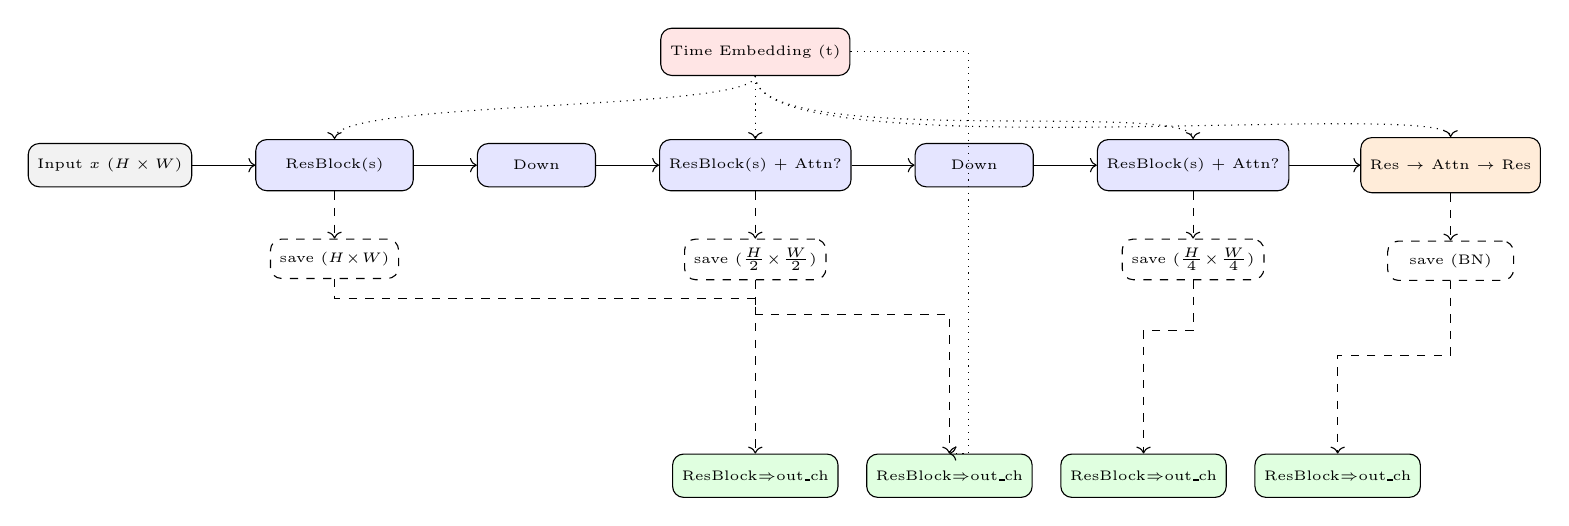
\begin{tikzpicture}[every node/.style={font=\tiny}]
% 输入
\node[draw, rounded corners, minimum width=1.9cm, minimum height=0.55cm, fill=gray!10]
  (inp) {Input $x$ ($H\times W$)};

% 第一层
\node[draw, rounded corners, minimum width=2.0cm, minimum height=0.65cm, right=0.8cm of inp, fill=blue!10]
  (l1) {ResBlock(s)};
\draw[->] (inp) -- (l1);

% 下采样1前快照
\node[draw, dashed, rounded corners, minimum width=1.6cm, minimum height=0.5cm, below=0.6cm of l1, fill=white]
  (s1) {save $(H\!\times\! W)$};
\draw[->, dashed] (l1.south) -- (s1.north);

% 下采样1
\node[draw, rounded corners, minimum width=1.5cm, minimum height=0.55cm, right=0.8cm of l1, fill=blue!10]
  (down1) {Down};
\draw[->] (l1) -- (down1);

% 第二层(含注意力)
\node[draw, rounded corners, minimum width=2.1cm, minimum height=0.65cm, right=0.8cm of down1, fill=blue!10]
  (l2) {ResBlock(s) + Attn?};
\draw[->] (down1) -- (l2);

\node[draw, dashed, rounded corners, minimum width=1.6cm, minimum height=0.5cm, below=0.6cm of l2, fill=white]
  (s2) {save $(\frac{H}{2}\!\times\!\frac{W}{2})$};
\draw[->, dashed] (l2.south) -- (s2.north);

% 下采样2
\node[draw, rounded corners, minimum width=1.5cm, minimum height=0.55cm, right=0.8cm of l2, fill=blue!10]
  (down2) {Down};
\draw[->] (l2) -- (down2);

% 第三层
\node[draw, rounded corners, minimum width=2.0cm, minimum height=0.65cm, right=0.8cm of down2, fill=blue!10]
  (l3) {ResBlock(s) + Attn?};
\draw[->] (down2) -- (l3);

\node[draw, dashed, rounded corners, minimum width=1.8cm, minimum height=0.5cm, below=0.6cm of l3, fill=white]
  (s3) {save $(\frac{H}{4}\!\times\!\frac{W}{4})$};
\draw[->, dashed] (l3.south) -- (s3.north);

% bottleneck
\node[draw, rounded corners, minimum width=2.1cm, minimum height=0.7cm, right=0.9cm of l3, fill=orange!15]
  (mid) {Res $\rightarrow$ Attn $\rightarrow$ Res};
\draw[->] (l3) -- (mid);

\node[draw, dashed, rounded corners, minimum width=1.6cm, minimum height=0.5cm, below=0.6cm of mid, fill=white]
  (sb) {save (BN)};
\draw[->, dashed] (mid.south) -- (sb.north);

% fea_tran heads(压到更近的位置)
\node[draw, rounded corners, minimum width=1.7cm, minimum height=0.55cm, below=2.2cm of s2, fill=green!12]
  (head1) {ResBlock$\Rightarrow$out\_ch};
\node[draw, rounded corners, minimum width=1.7cm, minimum height=0.55cm, right=0.35cm of head1, fill=green!12]
  (head2) {ResBlock$\Rightarrow$out\_ch};
\node[draw, rounded corners, minimum width=1.7cm, minimum height=0.55cm, right=0.35cm of head2, fill=green!12]
  (head3) {ResBlock$\Rightarrow$out\_ch};
\node[draw, rounded corners, minimum width=1.7cm, minimum height=0.55cm, right=0.35cm of head3, fill=green!12]
  (headb) {ResBlock$\Rightarrow$out\_ch};

\draw[->, dashed] (s1) -- ++(0,-0.5) -| (head1.north);
\draw[->, dashed] (s2) -- ++(0,-0.7) -| (head2.north);
\draw[->, dashed] (s3) -- ++(0,-0.9) -| (head3.north);
\draw[->, dashed] (sb) -- ++(0,-1.2) -| (headb.north);

% time embedding(上置且连线更紧凑)
\node[draw, rounded corners, minimum width=2.0cm, minimum height=0.6cm, above=0.8cm of l2, fill=red!10]
  (temb) {Time Embedding (t)};

\draw[->, dotted] (temb.south) .. controls +(0,-0.45) and +(0,0.5) .. (l1.north);
\draw[->, dotted] (temb.south) .. controls +(0,-0.7) and +(0,0.5) .. (l2.north);
\draw[->, dotted] (temb.south) .. controls +(0,-0.95) and +(0,0.5) .. (l3.north);
\draw[->, dotted] (temb.south) .. controls +(0,-1.2) and +(0,0.5) .. (mid.north);
\draw[->, dotted] (temb.east) -- ++(1.5,0) |- (head2.north);
\end{tikzpicture}
}% end resizebox
\vspace{2pt}

\footnotesize \textit{注:虚线箭头表示“保存该尺度特征”;点划线表示时间嵌入注入。}
\end{frame}
\begin{frame}[standout]
  谢谢大家!
\end{frame}
\end{document}
